\lysh{25461}{4}
\begin{alist}
\item Από τη γραφική παράσταση της συνάρτησης $f'$ συμπεραίνουμε ότι:
\[ f'(x) = 0 \Leftrightarrow x = 0 \text{ ή } x = 3 \]
\[ f'(x) > 0 \Leftrightarrow x \in (0,3) \]
\[ f'(x) < 0 \Leftrightarrow x \in (-\infty,0) \cup (3,+\infty) \]
Τα πρόσημα της παραγώγου της $f$ φαίνονται στον ακόλουθο πίνακα:

\begin{center}
\begin{tikzpicture}
\tikzset{arrow style/.style={maincolor,>->,>=latex'}}
\tikzset{t style/.style = {style = dashed}}
\tikzset{z style/.style = {fill=white,inner sep=.2mm}}
\tkzTabInit[color,lgt=2,espcl=2.4,colorC = maincolor!50,colorL = maincolor!30,colorV = maincolor!50]%
{$x$ / .8, $f'(x)$ /.8, $f(x)$/0.8}%
{$-\infty$, $0$, $3$, $+\infty$}%
\tkzTabLine{ , -, z, +, z, -, }
\tkzTabVar{+/ , -/ , +/ , -/ }
\end{tikzpicture}
\end{center}

Άρα, η συνάρτηση $f$ είναι γνησίως φθίνουσα στα διαστήματα $(-\infty,0]$ και $[3,+\infty)$ και γνησίως αύξουσα στο διάστημα $[0,3]$.

\item Η συνάρτηση $f$ είναι γνησίως αύξουσα στο διάστημα $[0,3]$ και, αφού είναι $1 < 2$, θα ισχύει $f(1) < f(2)$.

\item Αφού η γραφική παράσταση της συνάρτησης $f$ διέρχεται από τα σημεία $A(0,-1)$ και $B(3,2)$, τότε θα είναι:
\[ f(0) = -1 \quad \text{και} \quad f(3) = 2 \]

Από τον πίνακα του ερωτήματος (α) προκύπτει ότι η συνάρτηση $f$ παρουσιάζει τοπικό ελάχιστο για $x = 0$, το οποίο ισούται με $f(0) = -1$ και τοπικό μέγιστο για $x = 3$, το οποίο ισούται με $f(3) = 2$.
\end{alist}
\vspace{6mm}
\noindent\rule{\textwidth}{0.4pt}
\vspace{6mm}

